\ifx\wholebook\relax \else

\documentclass[b5paper]{ctexart}
\usepackage[nomarginpar
  %, margin=.5in
]{geometry}

\addtolength{\oddsidemargin}{-0.05in}
\addtolength{\evensidemargin}{-0.05in}
\addtolength{\textwidth}{0.1in}

\usepackage[cn]{../prelude}

\setcounter{page}{1}

\begin{document}

\title{复数}

\author{刘新宇
\thanks{{\bfseries 刘新宇} \newline
  Email: liuxinyu99@hotmail.com \newline}
  }

\maketitle
\fi

\markboth{复数}{数的旅程}

\ifx\wholebook\relax
\chapter{复数}
\fi

%% On earth there is nothing great but man; and in man there is nothing great but mind.
\epigraph{地球上最伟大的是人,人之中最伟大的是心灵}{威廉·汉密尔顿}

读过金庸武侠小说的读者一定对“华山论剑”津津乐道。天下武林中的顶级高手约定在华山比武论剑。大家各自身怀秘不外传的绝世武功,通过比武确定谁是真正的天下武功第一。十六世纪的意大利也上演了精彩的华山论剑。只不过没有刀光剑影、没有拳脚身法,而是一场关于数学与荣誉的挑战。1535年2月13日深夜,塔尔塔利亚在威尼斯的家中踱来踱去,为即将到来的挑战苦思冥想。文艺复兴时期的意大利,学着间经常进行骑士般的公开挑战。这种挑战并不使用刀剑或者火枪进行决斗,双方各自向对方提出同等数目的数学题目,并在规定的时间内作答。正确答出多的人获胜。胜利的一方赢得荣誉或一定数目的奖金。这种一对一的“单挑”发生在知名学者之间,通常在大教堂这类城市公共场所进行,引起众人的围观。有时甚至市长或者贵族也会前来观看,因而使得胜负具有非常的意义,影响双方的社会地位、学术评价甚至职业发展。

例如1225年,神圣罗马帝国皇帝腓特烈二世在西西里行宫接见了斐波那契。宫廷学者看不起商人出身的数学家,于是向斐波那契发起了挑战。斐波那契成功解决了全部问题,为自己赢得了荣誉。这些题目中包含了一道一元三次方程\footnote{当时还没有代数符号,是用文字描述的,如:找到一个数,其立方加上其平方的两倍再加上其十倍是二十。}:\[x^3 + 2x^2 + 10x = 20\]

斐波那契使用古巴比伦的60进制数值解法给出了正确答案:
\[
1^022^{I}7^{II}42^{III}33^{IV}4^{V}40^{VI} = 1 + \frac{22}{60} + \frac{7}{60^2} + \frac{42}{60^3} + \dotsb
\]

相当于十进制小数1.3688081075,精确到了小数点后9位。这种公开挑战也造成了一种奇特现象:学者们把自己的研究成果视为高度机密。因为这样可以使得他在与别人的挑战中获得优势。一旦泄露,对方就能解出自己提出的问题。学者们在生前不发表自己的成果,而是在死前传给自己信任的门生。这在“不发表就发霉”的今天是很难理解的\cite{HanXueTao2012}。

塔尔塔利亚面临的挑战就是关于三次方程的,对手名叫费奥尔\footnote{安东尼奥・马里亚・费奥尔,Antonio Maria Fior}。尽管古巴比伦人在公元前2500左右就掌握了一元二次方程的解法,但人们在接下来的4000多年一直没有突破一般三次方程的解法。人们并不满足于斐波那契的数值解法,而希望得到如二次方程那样的求根公式。所谓\underdot{一般}是指形如$ax^3 + bx^2 + cx + d = 0$的三次方程,简单的特殊三次方程,如$x^3 = a$自然容易解出一个\footnote{另外两个根是复数:$\dfrac{-1 \pm i\sqrt{3}}{2}\sqrt[3]{a}$}根$x = \sqrt[3]{a}$。塔尔塔利亚经过自己的努力,独立发现了形如$x^3 + ax^2 = b$这种特殊三次方程的解。

但费奥尔不断向世人吹嘘他会解三次方程,是意大利最好的学者,并向塔尔塔利亚发起挑战。双方约定各出30道题目,用火漆封好,在教堂决出谁更优秀。塔尔塔利亚心中忐忑不安。从费奥尔向别人炫耀的题目中,他隐隐感觉到费奥尔所能解出的三次方程不是$x^3 + ax^2 = b$,而是另一种形式:$x^3 + ax = b$,例如:“找到一个数,把它的立方加到自身上等于6”(相当于$x^3 + x = 6$)。但塔尔塔利亚却不知道如何解出这种方程\cite{MacTour-Tartaglia-Cardan}。他为此辗转反侧,茶饭不思。他思绪万千,童年时的一幕幕不断闪现在脑海中。

\index{数学家!塔尔塔利亚}
塔尔塔利亚原名尼科洛・丰塔纳,1499年或1500年,他出生于意大利的布雷西亚。父亲米凯莱·丰塔纳是一名邮递员,在布雷西亚周边的山区送邮件。家中有两男一女三个孩子,生活贫苦。尼科洛6岁时,父亲在送信的路上被人谋杀。失去了顶梁柱,全家陷入了极度贫困。更可怕的灾难还在后面。1512年,法军进攻布雷西亚\footnote{1494~1559年爆发了意大利战争。法国国王路易十二企图征服意大利,这遭到了西班牙哈布斯堡王朝等欧洲列强的反对,引发了战争。},为了报复布雷西亚人的坚决抵抗,法军在攻占后杀死了4.6万人。母亲带着尼科洛和妹妹想躲进教堂避难,但尼科洛还是在混乱中被一名法国士兵砍伤了面部,嘴巴上有两道触目惊心的伤痕。母亲找到了奄奄一息的孩子,但却没有钱请医生,她只好每天给他舔舐伤口。尼科洛奇迹般地活了下来,但是却因伤终身口吃。为此他得到了一个外号“小结巴”,塔尔塔利亚就是意大利语结巴的意思。他年长后一直留着胡子以遮掩脸上的伤疤。

尽管遭遇了诸多不幸,塔尔塔利亚却展现出了学习的天赋。他基本靠自学,买不起纸就用墓碑当作石板来代替。后来母亲终于找到了一位好心人资助他去帕多瓦学习。学成后塔尔塔利亚在维罗纳成了一名小学数学教师。1534年他搬到威尼斯,在圣扎诺波洛教堂教数学。此后他通过赢得一系列的公开挑战越来越有名气\cite{MacTour-Tartaglia}。往事如烟,现在塔尔塔利亚必须集中精神,尽快解决不含有二次项的三次方程。这个晚上,奇迹发生了,他终于找到了解法。当双方撕开火漆密封的题目,其实胜负已分:塔尔塔利亚的30道题目包含了两种特殊的三次方程,既有不含一次项的,也有不含二次项的;而费奥尔的只有不含二次项的一种。塔尔塔利亚只用了两个小时就正确解出了全部题目,但费奥尔被不含一次项的方程困住了。


\index{数额家!卡尔达诺}

\begin{figure}[htbp]
  \centering
  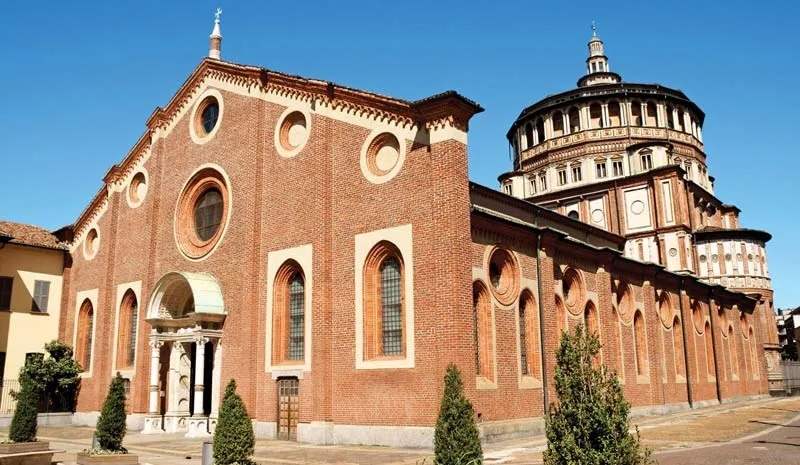
\includegraphics[scale=0.33]{img/churchmilan}
  \caption{米兰圣母玛丽亚感恩大教堂}
 \label{fig:church-Milan}
\end{figure}

%% del Ferro:德尔・费罗(意大利数学家尼科洛・德尔・费罗,Niccolò del Ferro,15 世纪末至 16 世纪初,首次解出一元三次方程的一类特殊情况)
%% Ferrari:费拉里(意大利数学家洛多维科・费拉里,Lodovico Ferrari,16 世纪,在卡尔达诺指导下首次解出一元四次方程)

\section{三次方程}

\begin{figure}[htbp]
  \centering
  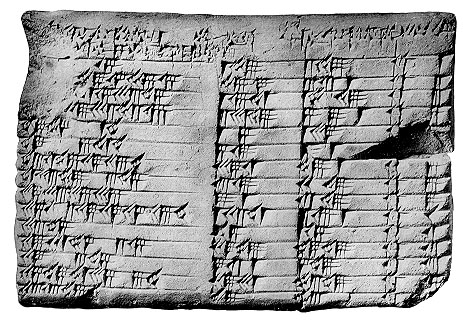
\includegraphics[scale=0.33]{img/plimpton322}
  \caption{编号普林普顿322的古巴比伦泥板,内容为勾股数表,约公元前2020年。藏于哥伦比亚大学。二十世纪二十年代由乔治·亚瑟、普林普顿捐赠给哥伦比亚大学。}
 \label{fig:plimpton322}
\end{figure}

解三次方程的历史

\section{佚名数学家}
\subsection{复数的几何意义和运算法则}
\subsection{匿名作者阿尔冈}
\subsection{代数基本定理}

\section{e的传奇}
\subsection{e的诞生}
\subsection{最美公式}

\section{新世界的大门}
\subsection{小试牛刀}
麦钦公式、正五边形作图
\subsection{费马大定理与高斯整数}
\subsection{抽象的数}
理想数
\subsection{新数的构造-代数数}

\ifx\wholebook\relax \else
\section{参考答案}
\shipoutAnswer

\begin{thebibliography}{99}
\subimport{inc/}{bib-zh-cn}
\end{thebibliography}

\expandafter\enddocument
\fi
